
%
%  $Description: Author guidelines and sample document in LaTeX 2.09$ 
%
%  $Author: ienne $
%  $Date: 1995/09/15 15:20:59 $
%  $Revision: 1.4 $
%

\documentclass[times, 10pt,twocolumn]{article} 
\usepackage{latex8}
\usepackage[utf8]{inputenc}
\usepackage{times}
\usepackage{graphicx}

%\documentstyle[times,art10,twocolumn,latex8]{article}

%------------------------------------------------------------------------- 
% take the % away on next line to produce the final camera-ready version 
\pagestyle{empty}

%------------------------------------------------------------------------- 
\begin{document}

\title{\LaTeX\ Author Guidelines 
       for {\boldmath $8.5 \times 11$-Inch} Proceedings Manuscripts}

\author{Miguel Belém\\
83531\\
% For a paper whose authors are all at the same institution, 
% omit the following lines up until the closing ``}''.
% Additional authors and addresses can be added with ``\and'', 
% just like the second author.
\and
Tiago Gonçalves\\
83567\\
\and
Vítor Nunes\\
83576\\
}

\maketitle
\thispagestyle{empty}

\begin{abstract}
   In this project we will apply two different aproaches to solve the problem of
   having a distributed tupplespace. 
   These aproaches have different tradeoffs considerations regarding time spent 
   executing a request, network congestion and time spent recovering from a fault.
   For this work we consider a perfect failure detector, in which if a server stop
   responding to requests, then is because it crashed.   
\end{abstract}



%------------------------------------------------------------------------- 
\Section{Introduction}

%Please follow the steps outlined below when submitting your 
%manuscript to the IEEE Computer Society Press. Note there have 
%been some changes to the measurements from previous instructions.
A tuple space consists in distributed collection of tuples. A tuple contains
fields that are some how related.
A basic tuple space needs to be writable, readable and deletable.

\textbf{Challenges.} At a first glace seems easy to implement a tuple space
in a distributed way however problems like consistency, data loss and 
performance rise.

To overcome this challenges we propose two diferent implementations of a 
distributed tuple space which solve the challenges listed above.

The State Machine Replication (SMR) which uses a coordination mechanism envolving
one leader to be responsible for coordination.

And a Xu and Liskov implementation that discards the need of a leader to
coordinate client's requests.


%------------------------------------------------------------------------- 
\Section{State Machine Replcation}

\begin{figure}
   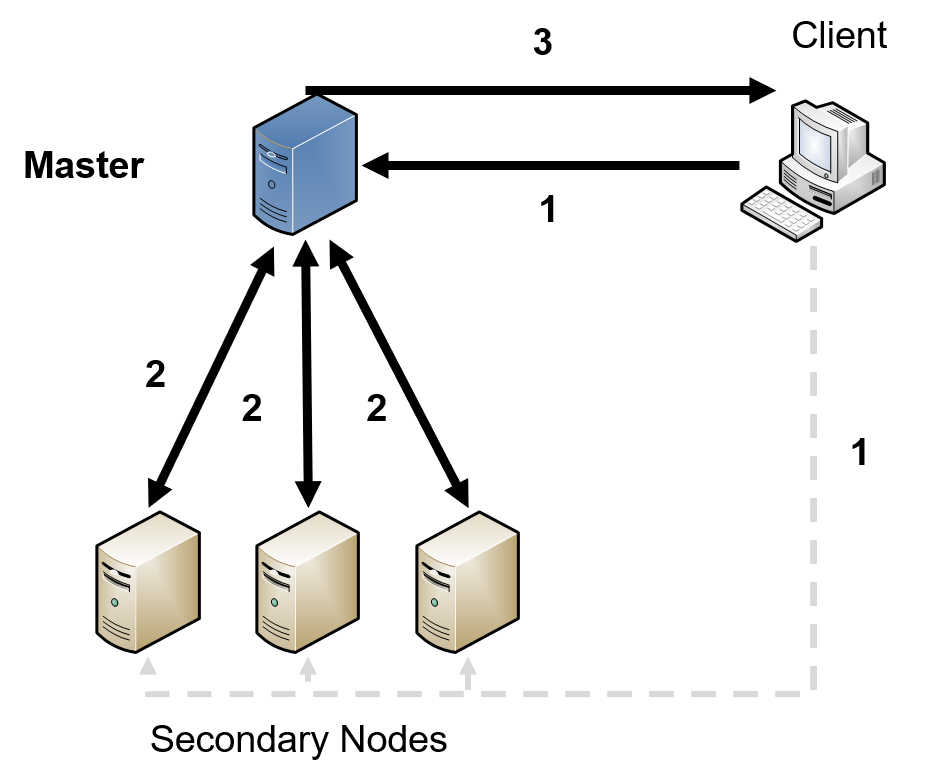
\includegraphics[width=\linewidth]{smr_basic.png}
   \caption{SMR basic communication schema}
   \label{fig:smr_basic}
 \end{figure}

The State Machine Replication is based on primary backup approach. Given one
primary and several secondary nodes, clients will perform requests to the
primary node only.

When the first server is switched on, we start by searching for alive servers
requesting \textsc{AreYouTheMaster}. If no reply is given then the server
becomes the leader. When others servers join the process repeats but they
will receive the reply containing the URL path of the master.

%------------------------------------------------------------------------- 
\SubSection{Clients request}

In our solution when the client starts we begin with a list of all URL's servers,
sends the request to all servers and only the leader will start processing, others
simply discard the request.

%------------------------------------------------------------------------- 
\SubSection{Fault tolerance}

\begin{figure}
   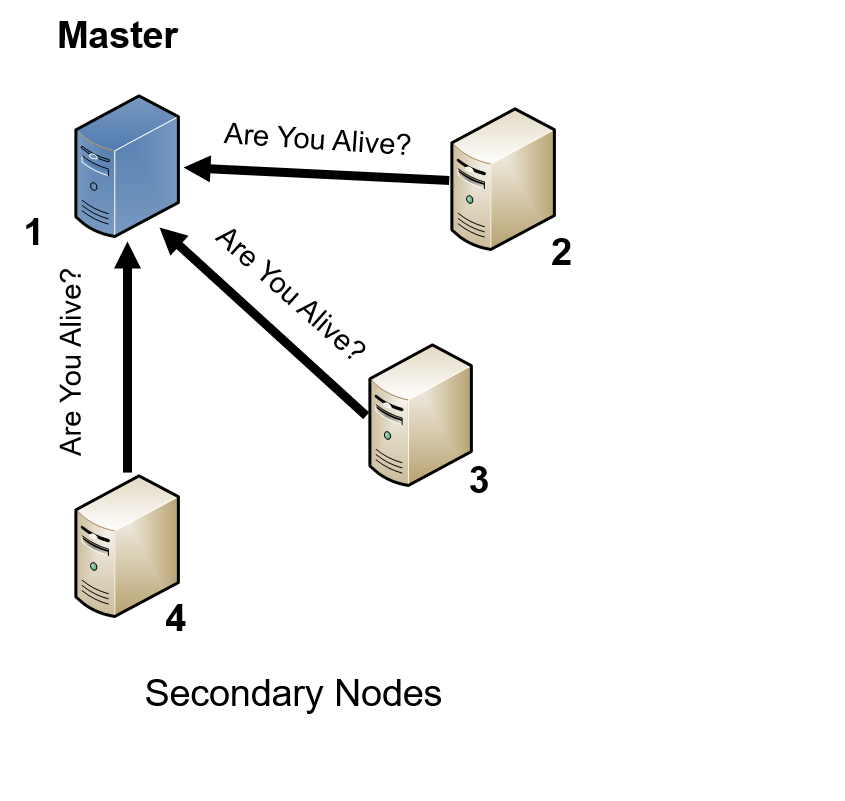
\includegraphics[width=\linewidth]{smr_ping.png}
   \caption{SMR master failure detector}
   \label{fig:smr_ping}
 \end{figure}

 \begin{figure}
   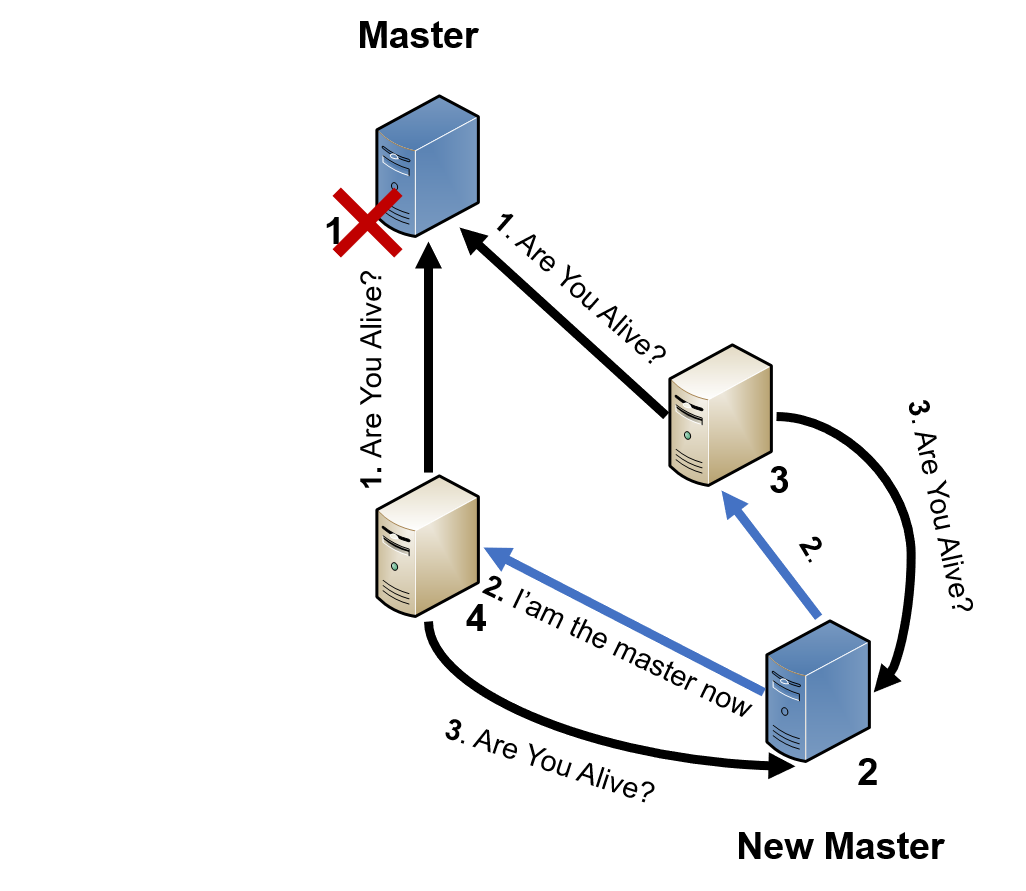
\includegraphics[width=\linewidth]{smr_master_recover.png}
   \caption{SMR master failure and system's recovering process}
   \label{fig:smr_master_recover}
 \end{figure}

This implementation has an obvious \textbf{week point}: if the master crashes 
the system will stop repling to requests.
Our solution to this problem consists of using an heartbeat that is sent from the
secondary nodes to the primary node every random seconds between 3 to 10 seconds.
This ensures that in the worst case the system will took ten seconds to
recovers (assuming instant propagation of messages) . 
The randomization process is used to optimize network bandwith and
prevent heartbeats flooding on the master.

Every node in the SMR contains an identifier. When a master crashes the remaining
node with the smallest ID will be elect as the new master. It starts by informing
all secondary nodes about its leadership change. By that time all secondary nodes
start sending heartbeets to the new master.

Another problem is when a \textbf{secondary node crashes}. In this case the
availability of the system is not affected since the primary node continues 
to receive client's request. Nevertheless if that same node resurrects then it
will be unconsistent with others. To fix this problem, every node has a log.

A log is used to keep track of every request made by the master 
\textbf{that was already executed.} When a secondary node crashes and recovers
it will have no such tuple in the tuple space, then request to the master
a copy of his own log. The master suspend the client's requests processing and
replies to the new secondary node. As soon the new node is ready the master
continues to processing client's request.


%------------------------------------------------------------------------- 
\Section{Xu and Liskov}

De acordo com esta implementação já não se recorre a um master que garante a 
consistência do sistema coordenando todos os pedidos. Em vez disso,
cada Front end de cada cliente vai propagar o pedido para todos os servidores vivos,
e cada um desses servidores vai tratar de o executar.
A Client's Front End is an interface to coordinate request to all nodes and made
them transparent to the user. For example, user invoke Front End's take operation
and FE is responsible for getting the current view and propagate the request
to multiple nodes.

%------------------------------------------------------------------------- 
\SubSection{Clients request}

%Na nossa solução, quando um cliente quer realizar uma lista de um ou mais pedidos,
%vai inicialmente criar um Front End, que vai procurar quais os servidores vivos,
%e com isso é criada a View do cliente, que tem um ID. 
%Quando um pedido é enviado para os servidores, é anexado ao mesmo o ID da view do cliente,
%o que permite ao servidor saber se a view do cliente está ou não sincronizada com as views
%dos servidores, caso não esteja, é porque o sistema sofreu uma modificação e quando recuperar da mesma,
%a nova é enviada ao cliente.

In this approach, when a client wants to perform some operation, stats by creating
a Front End. The client reads the server's URL path from the file and asks for
the view.

When a request \textsc{Read}, \textsc{Write} or \textsc{Take} is sent to the servers,
it is checked server-side if the view is up-to-date.
The server will only execute the request if the view is the most recent. Otherwise
simply returns null and forces the client to update its view first and repeat the
request.

Every view contains a \textbf{version} which allows compare two views and determine the
most recent view. When a client starts up we gets one view from the server before
making requests to the client.

The \textbf{biggest advantage} over our SMR implementation is that the client will only
send requests to servers that are supose to be alive.

%------------------------------------------------------------------------- 
 
\SubSection{Fault tolerance}


\begin{figure}
   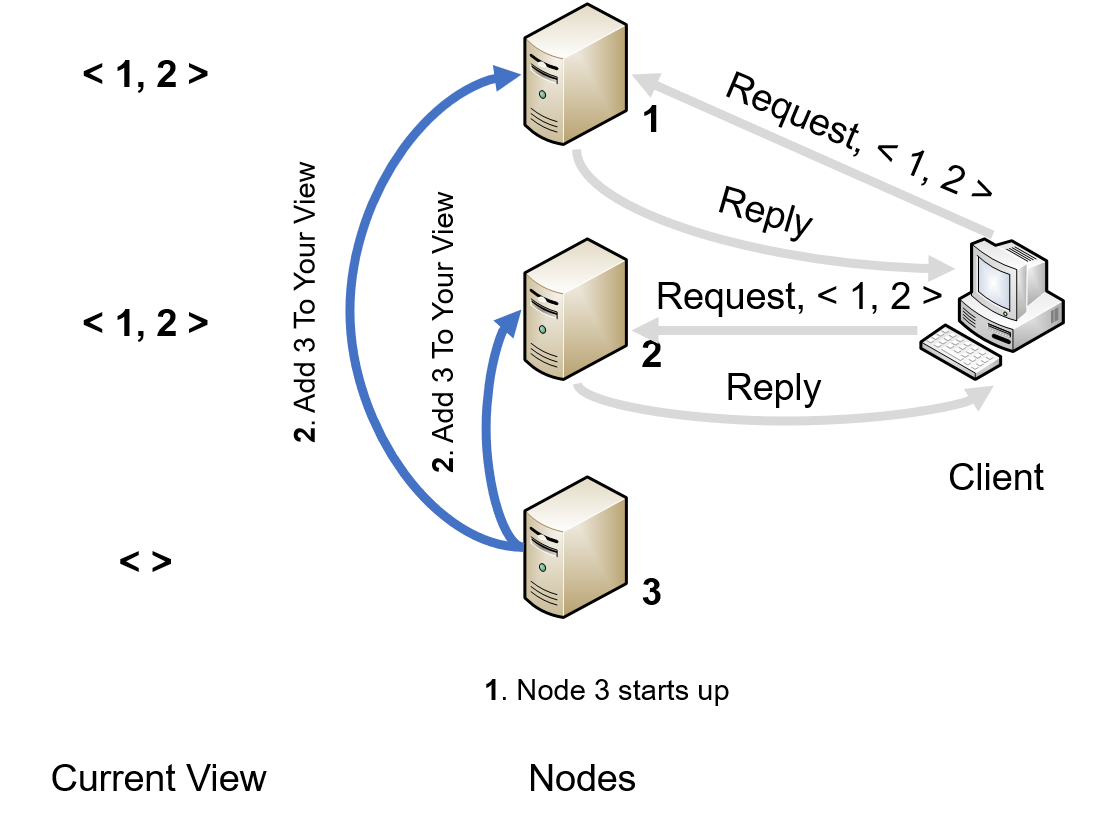
\includegraphics[width=\linewidth]{xl_join1.png}
   \caption{XL view update process}
   \label{fig:xl_join1}
 \end{figure}

\begin{figure}
   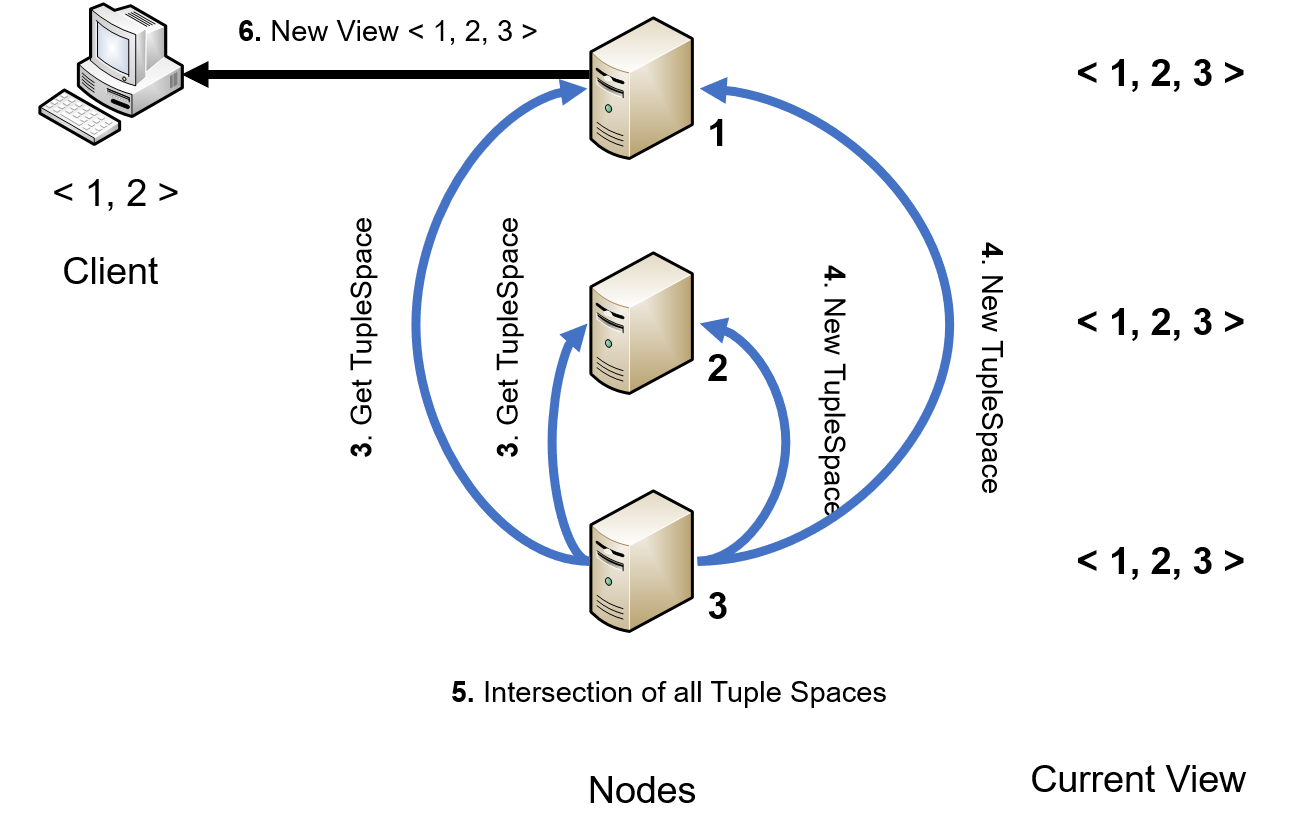
\includegraphics[width=\linewidth]{xl_join2.png}
   \caption{XL tuple space recover}
   \label{fig:xl_join2}
 \end{figure}

%Esta abordagem, ao não apresentar um master, tem a vantagem de que quando um nó crasha,
%seja ele qual for, o sistema não precisa de parar. Isto é possível pois não existe uma
%unidade central da qual todo o sistema dependa, e que caso a mesma crashe, todo o sistema 
%é comprometido.

This approach has an advantage of time in recovering, this happens because when
a node crashes the system don't need to stop. There are no coordinator node
(a central point of failure) that could compromise the system availability.

%Apresenta uma desvantagem em relação ao SMR que é a de precisar de parar o sistema por 
%breves instantes quando um novo nó se liga ao sistema. Isto é feito pois as Views precisam
%de ser atualizadas para passar a conter o novo nó, e não se podem perder pedidos que
%estejam a ser feitos enquanto as Views são atualizadas.

However has the following \textbf{pitfall}: when a new node joins it is necessary
to pause the entire system to performe a view update in order to ensure consistency
and garantee that the clients request during the view update will not disapear.

The following steps are executed when a node crashes:
\begin{itemize}
   \item Client suspend all requests
   \item Client detects the crash and inform all other view members
   \item Client resume the requests
\end{itemize}

Quando um nó crasha o cliente vai atualizar a sua view, e informar todos os seus membros
para atualizarem a deles.


%Quando um nó rescuscita, vai começar por informar todas as máquinas vivas de que precisa
%do seu espaço de tuplos e vai pedir para que atualizem as suas views. Cada máquina ao
%receber este pedido vai recusar pedidos dos clientes que apresentem uma view antiga
%e vai dar o seu tuplespace ao novo nó. 
%O novo nó vai fazer uma interseção de todos os tuplespaces (a interseção garante
%que ele apenas vai guardar os pedidos que já foram executados em todas as máquinas).
%Em seguida esse tuplespace é propagado para todo o sistema, com isto garantimos que 
%nunca se perdem pedidos, pois mesmo que um pedido já tenha sido enviado para uma máquina
%mas não para outra, vai acabar ser repetido. Após todos os tuplespaces terem sido
%atualizados, o novo nó sinaliza as outras máquinas para que mandem a sua nova view ao cliente,
%repetindo o mesmo todos os pedidos da mesma operação que foram enviados numa view antiga e que
%consequentemente foram recusados pelos servidores.

The following steps are executed when a new node joins the system:
\begin{itemize}
   \item New node starts up and for each path in file tries to update the view to inform his arrival
   \item As soon the already alive nodes receive a request to change the view they perform the request
   immediately and \textbf{do not send the new view to the client.} (Figure ~\ref{fig:xl_join1})
   \item All client's request are reject because the client view is out-of-date.
   \item New node request a copy of the tuple space to all already alive nodes.
   \item New node performs a tuple space intersection (see more in detail above) and propagates the changes
   to all already alive nodes. (Omitted on Figure ~\ref{fig:xl_join1} due to preserve draw simplicity)
   \item Only when the new tuple space is sent to all nodes then the client is informed of the new view. (Figure ~\ref{fig:xl_join2})
   \item The client can resume the requests to all nodes.   
\end{itemize}

\textbf{Tuple Space Intersection:} We defined a intersection of tuple space as the set of tuples
that belongs to both tuple spaces.

Let's supose, for example that we have \textbf{2 nodes already alive} and a new node joins the system.
The following schema shows the tuple space content of each node:

$ TupleSpace_{1} \leftarrow <dog, brown>, <cat, white>, <cat, gray> $

$ TupleSpace_{2} \leftarrow <dog, brown>, <cat, white>, <cat, gray>, <horse, white> $

$ TupleSpace_{3} \leftarrow \emptyset $

A closer look to $TupleSpace_{2}$ shows a partial write operation, this is
the client's front end wrote on node 2 but lost his view and therefore couldn't wrote on other nodes.

Remember that node 3 will request all tuples spaces (from node 1 and 2) and perform a intersection, this is:

$ TupleSpace_{3} \leftarrow TupleSpace_{1} \cup TupleSpace_{2} $

$ TupleSpace_{3} \leftarrow <dog, brown>, <cat, white>, <cat, gray>$

At a first glance seams like the new tuple $<horse, white>$ has been lost due 
to the expiration of the view. Nevertheless the client needs to perform the 
request again, and because of this the tuple will be added again.

This \textbf{garantees consistency} as the partial writes/takes will be discarded
and repeated as complete write/takes operations!

%------------------------------------------------------------------------- 
\Section{Evaluation}
%Nesta secção vamos analisar e avaliar como cada algorítmo se comporta no que toca 
%a alguns pontos chaves. Apresentamos ainda a justificação para algumas escolhas que
%tiveram de ser feitas.

In this section we will study how these approachs (SMR and XL) performs in some metrics.
We still present some justifications about concrete implementation aspects.

\SubSection{Requests execution}
\subsubsection{SMR}

%Para a operação de Take e Write é necessário que os pedidos cheguem ao master
%e depois este propaga para o resto dos servidores/réplicas. Isto além de sobrecarregar um servidor pois 
%é ele que tem de receber a transmitir os pedidos e posteriormente esperar pelas respostas 
%dadas pelas réplicas também atrasa a respostas aos pedidos pois é preciso que os mesmo passem
%por um intermediário.

For \textsc{Take} and \textsc{Write} operations it is necessary that the master receive the requests
and then propagate it tho secondary nodes. The biggest disadvantage of this approach is the extra
load that a master needs to handle, this is the client's and nodes requests/replies and even heartbeets.

%Na operação de Read os pedidos não são propagados pera as réplicas, devolvendo o master 
%instantâneamente a resposta ao cliente, caso seja possível (Take e Read são operações bloquentas, 
%para ser dada uma resposta é preciso que a mesma conste nos espaços de tuplos).

\textsc{Read} requests are the only type of client request that the master won't propagate to other nodes.
As soon the master receives the \textsc{Read} it respondes immediately to the client.


\subsubsection{XL}

%Para a operação Write o cliente propaga o pedido para todos os servidores. Para a operação de Read
%o cliente propaga o pedido para todos os servidores e devolve ao cliente quando obtiver a primeira
%resposta. Para a operação de Take foram tidos em conta alguns cuidados, nomeadamente: é necessário
%bloquear certas entradas do espaço de tuplos e convem que esta parte seja feita de uma maneira que 
%não obrigue a que o cliente fique muito tempo à espera de uma resposta assim sendo o algorítmo usado
%foi o de tentar bloquear tantas entradas que dêm match com o pedido quanto possível, e quando não for 
%ossível adquirir o trinco de uma dada entrada, o conjunto de entradas que cujo trinco foi adquirido
%sao devolvidas ao front end, em seguida o front end vai intersetar os conjuntos que recebeu dos vários
%servidores e vai escolher um elemento comum a todos esses conjuntos e remove-lo, devolvendo ao cliente.

For the \textsc{Write} operation the client's front end propagate the request to all alive servers.

The \textsc{Read} operation is performed by the front end and returns to the client the first response it gets.

The \textsc{Take} operation is a little bit more tricky, in the sense that has two phases:

\textbf{\textsc{Take} Phase 1}
\begin{itemize}
   \item Node receives a specific tuple object to be taken from the tuple space.
   \item Returns a list of all matching tuples and locks them on a lock list (see more details above)
   \item The client's front end performes a intersection operation on all responses of all nodes and sends the result
   back.
\end{itemize}

\textbf{\textsc{Take} Phase 2}
\begin{itemize}
   \item Node receives a specific tuple object to be taken from the tuple space.
   \item Removes that tuple.
   \item Unlocks all other tuples from the lock list.
\end{itemize}

\textbf{Lock List:} It is a log that creates a mapping between the client Id and the
tuples that are locked to that client during the \textsc{Take} Phase 1.

Every tuple can only be locked to a user at the same time.

% vitor: question
Esta foi a melhor solução encontrada, pois usamos uma heurística que tenta devolver o máximo de entradas
possível no entanto não fica muito tempo à espera de modo a conseguir todas a entradas possíveis (se existirem
muitos pedidos simultâneos e todos fizerem isto, o que vai aconter é o servidor não conseguir dar resposta a ninguém
e ficar muito lento), esta heurística também não se contenta apenas com uma resposta (caso só fosse devolvida uma entrada,
na parte da interseção, a probabilidade de a mesma ser nula seria muito elevada). Com esta heurística conseguimos
ter algum equilíbrio.


\SubSection{Comparison}

Para a operação Write é expectável que o XL a execute mais rapidamente.
Para a operação de Read é expectável que ambas as implementações tenham um tempo de execução semelhante.
Para a operação de Take se a máquina master tiver uma capacidade de processamente muito elevada (não entupir com
um elevado número de pedidos), acabamos por conseguir ter tempos de resposta mais baixos pois não ficamos dependentes
da operação de interseção, que pode falhar, tendo de ser repetido todo o processo.

\SubSection{Network congestion}
\subsubsection{SMR}

Quando é feito um pedido de execução de uma operação, este é propagado para todos os servidores. Aqueles que são réplicas
ignoram o pedido (só executam pedidos do master), o master quando recebe vai propagá-lo para as réplicas. A juntar a isto 
temos ainda mensagens a serem trocadas a cada 3 a 10 segundos de cada uma das réplicas para o master, para verificar se o mesmo
não crashou.
 
\subsubsection{XL}

No normal desenrolar do sistema, o pedido é propagado para todos os servidores na View do Front End do cliente, por norma os pedidos são feitos
uma única vez. Exceptuando os casos em que por algum motivo a interseção na operação Take falha, ou quando um novo servidor entra no sistema e 
o mesmo tem de parar para as Views serem atualizadas, pedidos enviados durante essa altura teem de ser repetidos.

\subsubsection{Comparison}

A implementação SMR congestiona muito mais a rede que a implementação XL. XL poderá congestionar mais a rede que o SMR no caso em que
a View tenha de ser alterada, existam muitos pedidos a ser feitos e todos vão ter de ser repetidos. 

\SubSection{Fault recovering}
\subsubsection{SMR}

No caso de existir um crash numa das réplicas, o sistema não fica comprometido e pode fluir normalmente. No caso de ser o master a crashar
os pedidos dos clientes vão para um buffer e não são executados até um novo Master ser eleito. Para eleição do novo master é usado um algoritmo
de leader election que escolhe a réplica que tenha um ID mais baixo.

\subsubsection{XL}

Quando alguns dos servidores crasha o sistema não para. Simplesmente quando um cliente deteta isso propaga a nova View para os servidores e 
deixa de fazer pedidos a quem crashou.

\subsubsection{Comparison}

Para o SMR quando o Master crasha o sistema preciso de algum tempo para recuperar. Para o XL isso nunca acontece. Por outro lado no caso do XL,
quando uma nova máquina se liga, o sistema tem de parar por causa da operação de interseção.
Dependendo do sistema que se pretende implementar pode ser mais vantajosa uma ou outra abordagem. No caso em que novas máquinas se estejam sempre
a ligar o SMR reage melhor, no caso em que existam crashs constantes o XL reage melhor porque não possui nenhuma unidade central de coordenação. 

\Section{Summary and conclusions}

%No algorítmo SMR não são usadas Views, provocando uma latência enorme em todas as comunicações servidor servidor
%e cliente servidor, pois é necessário estar sempre a verificar do ficheiro que máquinas estão vivas. Uma modificação futura a este
%trabalho seria implementar um sistema de Views semelhante ao existente no XL.
%Um outro problema que deveria ser resolvido na implementação de SMR usada seria diminuir as mensagens constantes das réplicas
%para o master para verificar se o mesmo está vivo. 
%Não é possível dizer qual dos algorítmos é melhor, ambos apresentam vantagens e desvantagens, será necessário ver com atenção
%os tópicos referentes à Evaluation, e conforme o intuíto do sistema a ser desenvolvido, aplicar o que melhor se adeque aos objetivos
%do sistema.

In the SMR implementation we didn't use Views, leading to a latency growth between all server<->server and client<->server communications. 
This occurs because we need to check the availability of all servers contained in the servers file, which contains both the alive and death 
servers. One further modification to ours SMR implementation is to apply Views like the ones used in XL. 
Another problem that should be fixed in SMR is the one regarding the constant messages exchange from all Replicas to the Master.
It's not possible to say which implementation is better, it is necessary do read carefully the evaluation topics written in the previous section,
and based on which are the the requirements for the new system, make a decision.

Alguns cenários exemplificativos:
-Sistema 1 -> Para o caso dos minutos finais de um leilão queremos ter um elevado throghput, nessa altura não deverão existir máquinas novas a 
quererem ligar-se ao sistema e caso alguma máquina crashe, o sistema não pode ficar bloqueado. Para este cenário será muito mais vantajoso a 
utilização do XL, pois a rede não é tão congestionada e os pedidos são executados mais rapidamente. 
-Sistema 2 -> Para uma arquiterura Peer to Peer, na qual novas máquinas estão sempre a existir vai ser mais lucrativo utilizar o SMR pois o sistema
não bloqueia com a entrada de novos nós.

%------------------------------------------------------------------------- 
\nocite{ex1,ex2}
\bibliographystyle{latex8}
\bibliography{latex8}

\end{document}

